\chapter{Constraining the equation of state with astrophysics}
%\chapter{Astrophysics around neutrons stars}
\chapterimage[width=15cm]{wordcloud/chap3b.png}

\subsection{Accretion disks}

Gravitational potential energy release
\be
\Delta E_{\mathrm{acc}} = \frac{G M m}{R} \sim 10^{20}  \left( \frac{10\km}{R} \right) \left( \frac{M}{\Msun} \right) \unitspace\erg\unitspace\g^{-1}
\ee

Roche Lobe \cite{PRP02} \cite{LL15}

LMXB \cite{TH06}

Hard and soft state \cite{HvdK89}
Alternates between these two states \cite{MDF14} \cite{DGK07}



\subsection{Between the disk and the star: boundary layers}

\be
\Omega(R) \approx \Omega_{\mathrm{K}}(R) = \left( \frac{G M}{R^3} \right)^{1/2}
\ee

Layer of thickness $b$ equals $\Omega(R + b) \approx \Omega_{\mathrm{K}}(R + b)$ that must slow down to $\Omega_{*}$.

Energy difference
\be
\dot{E} = \frac{1}{2} \Mdot R^2 (\Omega_{\mathrm{K}}^2 - \Omega_{*}^2) = 
\frac{1}{2} \Mdot \frac{GM}{R} \left[ 1 - \left(\frac{\Omega_*}{\Omega_{\mathrm{K}}} \right)^2 \right] 
\ee

Viscous torque $G_{\mathrm{T}} = \Mdot R^2 (\Omega_{\mathrm{K}} - \Omega_*)$
Hence,
\be
\dot{E} = \frac{1}{2} \frac{G M \Mdot}{R} \left( 1 - \frac{\Omega_*}{\Omega_{\mathrm{K}}} \right)^2
\ee


\section{X-ray bursts}
\subsection{Unstable thermonuclear burning on top of neutron stars}

\subsection{Constraining the size of bursting source}




%--------------------------------------------------
\section{Accretion}
%infalling matter leads to X-rays \cite{Lewin93}

\subsection{Source of energy}
In the heart of this whole problem is an astrophysical process called accretion.

Gravitational potential energy release
\be
\Delta E_{\mathrm{acc}} = \frac{G M m}{R} \sim 10^{20}  \left( \frac{10\km}{R} \right) \left( \frac{M}{\Msun} \right) \unitspace\erg\unitspace\g^{-1}
\ee

Eddington luminosity
\be
L_{\mathrm{Edd}} = \frac{ 4 \pi G M \mproton c }{\sigma_{\mathrm{T}} } \approx \Ten{1.3}{38} \left( \frac{M}{\Msun} \right) \ergs
\ee

Accretion luminosity
\be
L_{\mathrm{acc}} = \frac{G M \Mdot}{R} 
\ee

\subsection{Binary systems}

\begin{figure}[t]
\centering
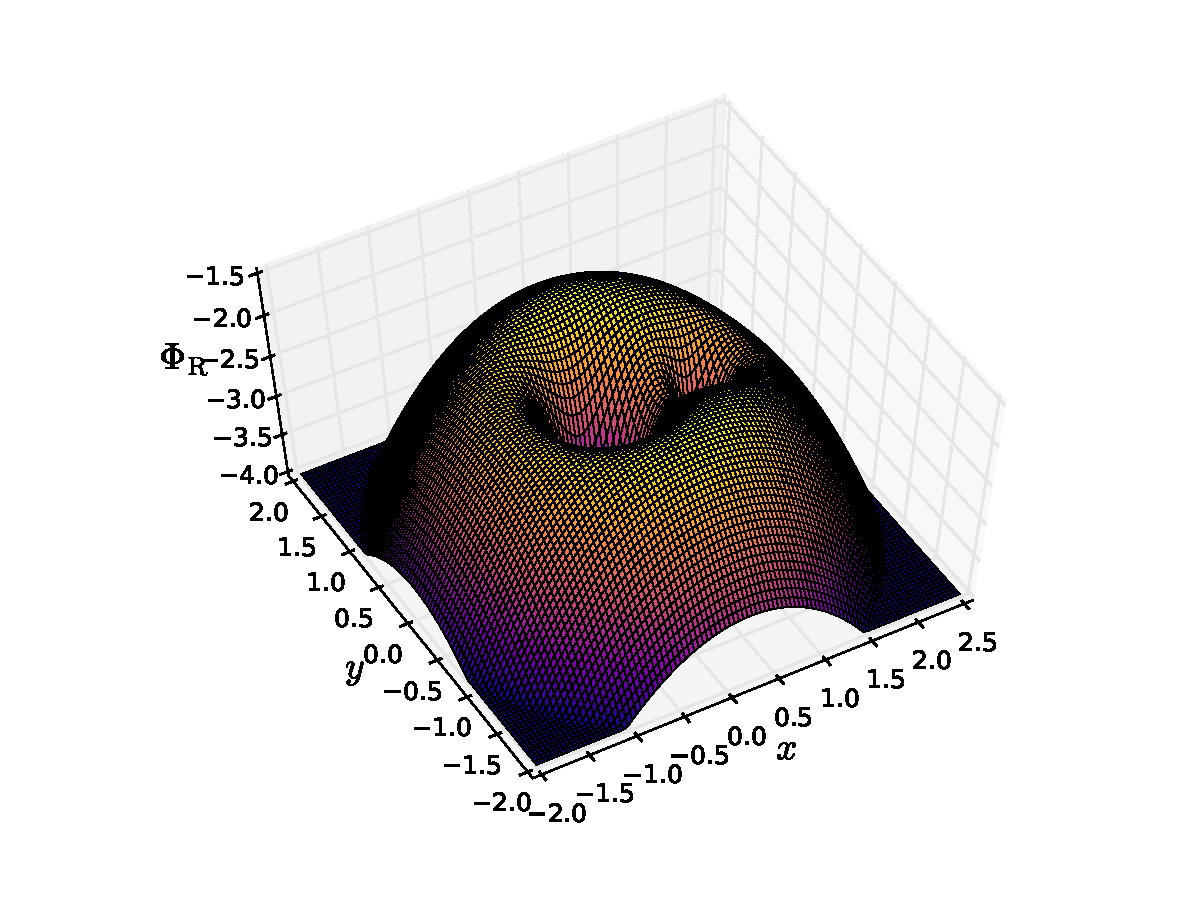
\includegraphics[width=7.5cm]{figs/astro/roche.pdf}
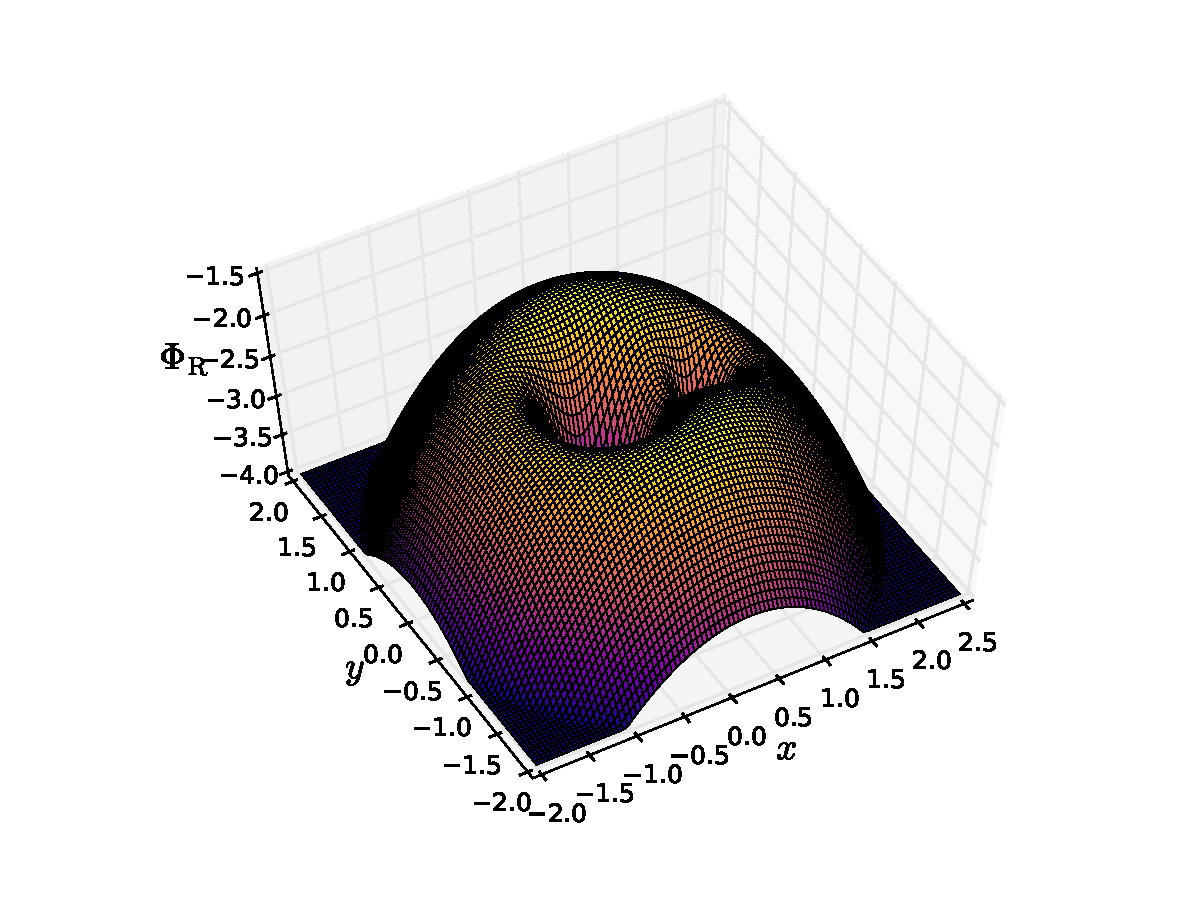
\includegraphics[width=7.5cm]{figs/astro/roche.pdf}
\caption{\label{fig:roche}
Roche potential for binary systems.
}
\end{figure}

\subsubsection{Roche lobes and mass transfer}
Roche Lobe \cite{PRP02} \cite{LL15}

A flow of gas between two stars can be described by the Euler equation.
It gives the time evolution of the velocity $\vec{v}$ of the gas that has a pressure of $P$ and density $\rho$.
In a reference frame rotating together with the binary system with angular velocity $\omega$ the Euler equation takes the form 
\be
\frac{ \partial \vec{v} }{\partial t} + (\vec{v} \cdot \nabla)\vec{v} = -\nabla \Phi_{\mathrm{R}} - 2 \vec{ \omega } \times \vec{v} - \frac{1}{\rho} \nabla P,
\ee
where the angular velocity of the binary is then
\be
\vec{ \omega } = \left( \frac{ G M }{a^3} \right)^{1/2} \vec{e},
\ee
as given with the unit vector $\vec{e}$, normal to the orbital plane.
Here $M$ is the total mass of the system, i.e. $M = M_1 + M_2$, where $M_1$ and $M_2$ are the individual masses of the two stars in the system, respectively, and $a$ is their orbital separation.

The effects originating from the gravitation and from the centrifugal forces are encapsulated in the so-called Roche potential, given as a function of radial vector $\vec{r}$ as
\be
\Phi_{\mathrm{R}}(\vec{r}) = -\frac{G M_1}{|\vec{r} - \vec{r_1}|} -\frac{G M_2}{|\vec{r} - \vec{r_2}|} - \frac{1}{2} ( \vec{ \omega } \times \vec{v} )^2,
\ee
where the location of the stars is given with $\vec{r_1}$ and $\vec{r_2}$.

By studying the shape of the potential, we see that in between the stars, in the so-called $L_1$ point there exists a location where the individual gravitational pull from the stars is balanced.
This leads to a kinda of a nozzle in the system from which the material can leak from the less massive star to the more massive object.
Such a leaking, or a Roche lobe overflow, will then occur if the companion star's radius exceeds the size of its Roche lobe.
Typically such a thing can happen when the star evolves and expands at the end of its life cycle. 

LMXB \cite{TH06}


\subsection{Accretion disks}
Hard and soft state \cite{HvdK89}
Alternates between these two states \cite{MDF14} \cite{DGK07}



\section{Accretion to a neutron star}

\subsection{Boundary layers}

\be
\Omega(R) \approx \Omega_{\mathrm{K}}(R) = \left( \frac{G M}{R^3} \right)^{1/2}
\ee

Layer of thickness $b$ equals $\Omega(R + b) \approx \Omega_{\mathrm{K}}(R + b)$ that must slow down to $\Omega_{*}$.

Energy difference
\be
\dot{E} = \frac{1}{2} \Mdot R^2 (\Omega_{\mathrm{K}}^2 - \Omega_{*}^2) = 
\frac{1}{2} \Mdot \frac{GM}{R} \left[ 1 - \left(\frac{\Omega_*}{\Omega_{\mathrm{K}}} \right)^2 \right] 
\ee

Viscous torque $G_{\mathrm{T}} = \Mdot R^2 (\Omega_{\mathrm{K}} - \Omega_*)$
Hence,
\be
\dot{E} = \frac{1}{2} \frac{G M \Mdot}{R} \left( 1 - \frac{\Omega_*}{\Omega_{\mathrm{K}}} \right)^2
\ee


\subsection{X-ray bursts}
Thermonuclear runaway.

\subsection{Constraining the size of the star}
Cooling tail method.





% --------------------------------------------------
\newpage
\section{Appendix A: Real astrophysics}

%\begin{itemize}
%    \item Accretion
%    \item Disks 
%    \item Soft and hard states
%    \item Boundary layers
%    \item Ignition?
%    \item X-ray bursts
%    \item Cooling tail method
%\end{itemize}
%
%Possible layout:
%
%v1
%\begin{enumerate}
%    \item Accretion
%    \begin{itemize}
%        \item Disks
%        \item Soft and hard states
%        \item Boundary layers
%    \end{itemize}
%    \item X-ray bursts
%    \begin{itemize}
%        \item Unstable thermonuclear burning
%        \item Cooling tail method
%    \end{itemize}
%\end{enumerate}
%
%v2
%\begin{enumerate}
%    \item Accretion disks
%    \begin{itemize}
%        \item Accretion
%        \item ?Roche lobe overflow
%        \item Soft and hard state
%        \item Boundary layers
%    \end{itemize}
%    \item X-ray bursts
%    \begin{itemize}
%        \item Unstable thermonuclear burning
%        \item Cooling tail method
%    \end{itemize}
%\end{enumerate}


\sect{Energetics}
Let us try and estimate the energetics of different phenomena of what we can observe from neutron stars.\mnote{Energy output}
Few possible stable sources of energy exists: thermal, gravitational, rotational, and magnetic.
In addition, unstable fusion processes can also power some observable phenomena.



